
%
%	Simulation
%

\section{Simulation}\label{Section_Simula}
\Headerfooter{Simulation}





\subsection{Atmospheric neutrino flux}
\vs\hs
Many hadrons like pions and kaons are generated by reactions between a cosmic ray and a nucleus in the atmosphere.
The generated hadron decays into a muon and a neutrino, and the muon decays into an electron and two neutrinos.
The generated neutrinos in the atmosphere are called ``atmospheric neutrinos''.
Figure~\ref{Simula_AtmNeu} shows the schematic view of atmospheric neutrino production.

\begin{figure}[h]
	\centering
	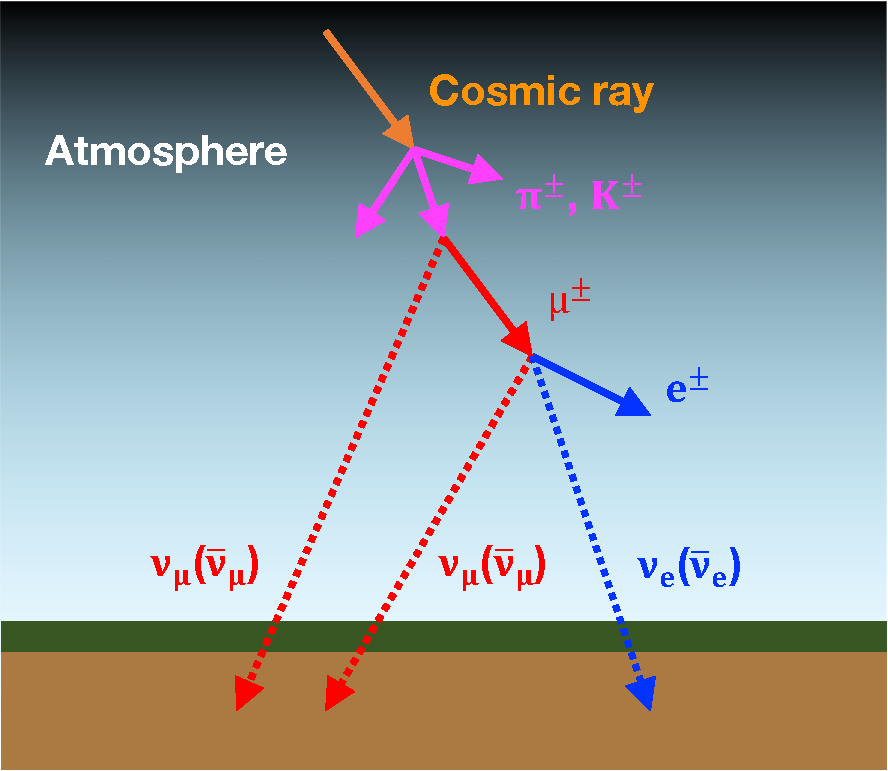
\includegraphics[width=6cm]{Figures/Simulation/AtmNeu}
	\caption[Schematic view of atmospheric neutrino production]{
	Schematic view of atmospheric neutrino production.
	}\label{Simula_AtmNeu}
\end{figure}

\hs
The atmospheric neutrino flux at the SK detector is predicted using the HKKM11 model~\cite{2011Honda}.
Figure~\ref{Simula_AtmNeuFlux} shows the atmospheric neutrino flux predicted by the HKKM11 model for the Kamioka site~\cite{2011Honda,2016Richard}.
As shown in this figure, the predicted flux shows good agreement with the observation in SK.
Atmospheric neutrino/antineutrino ratio and atmospheric neutrino flux of $\nu_{\rm e}\,+\,\nu_{\mu}$ ($\bar{\nu}_{\rm e}\,+\,\bar{\nu}_{\mu}$), $\nu_{\rm e}$ ($\bar{\nu}_{\rm e}$), and $\nu_{\mu}$ ($\bar{\nu}_{\mu}$) predicted by the HKKM11 model for the Kamioka site are shown in Figure~\ref{Simula_Ratio}~\cite{2011Honda}.
In this measurement, systematic uncertainties of atmospheric neutrino flux and atmospheric neutrino/antineutrino ratio are considered (see Section~\ref{SYSTEM}).

\begin{figure}[p]
	\centering
	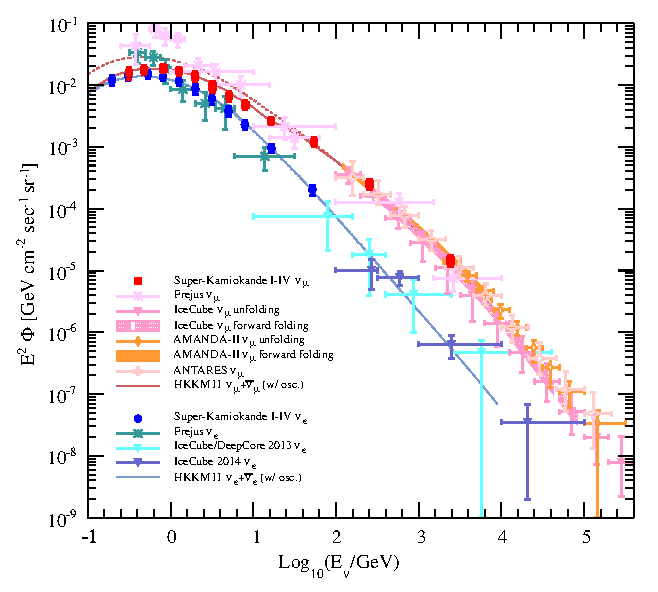
\includegraphics[width=8cm]{Figures/Simulation/AtmNeuFlux}
	\caption[Atmospheric neutrino flux predicted by the HKKM11 model for the Kamioka site]{
	Atmospheric neutrino flux predicted by the HKKM11 model for the Kamioka site~\cite{2011Honda,2016Richard}.
	Data plots are taken from the following experiments: Super-Kamiokande I-IV~\cite{2016Richard}, Frejus~\cite{1995Daum}, IceCube~\cite{2011Abbasi,2011Abbasi_02,2013Aartsen,2015Aartsen}, AMANDA-II~\cite{2009Abbasi,2010Abbasi}, and ANTARES~\cite{2013Adrian}.
	}\label{Simula_AtmNeuFlux}
\end{figure}

\begin{figure}[p]
	\centering
	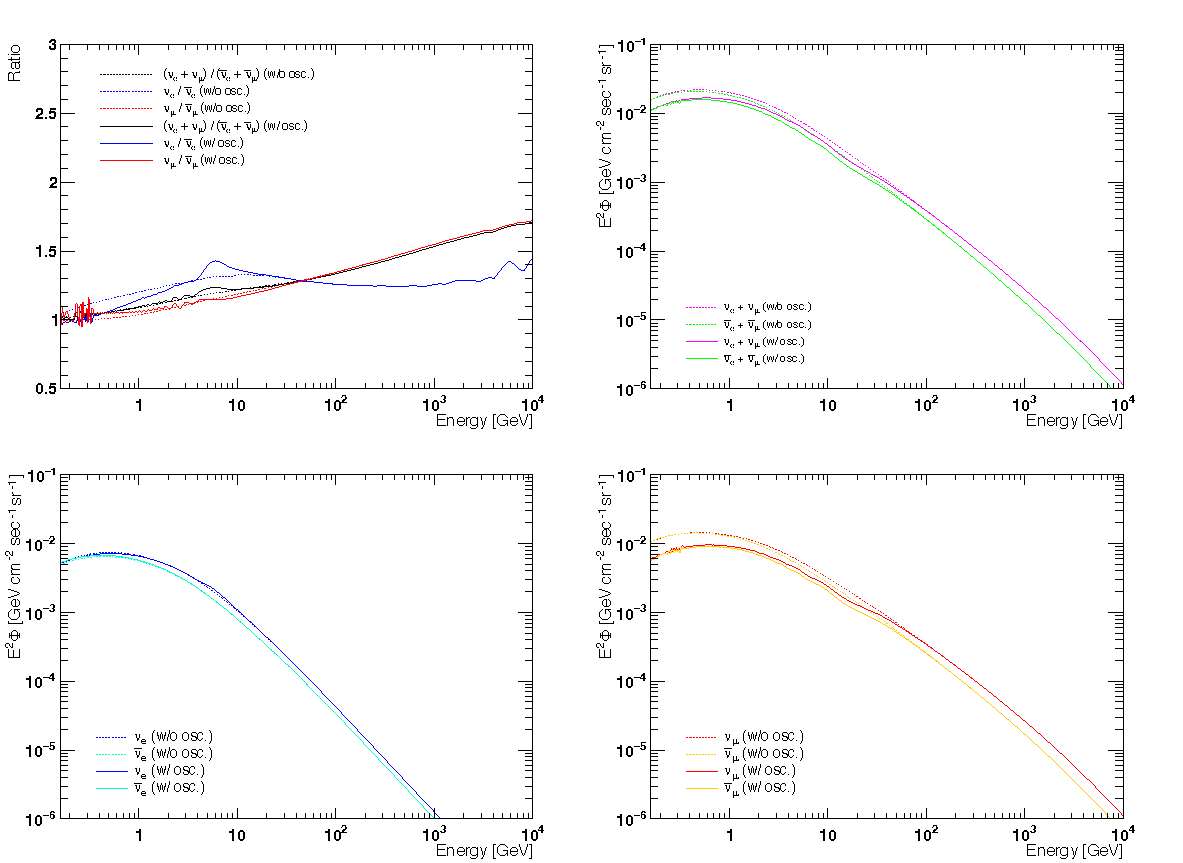
\includegraphics[width=16cm]{Figures/Simulation/Ratio}
	\caption[Atmospheric neutrino/antineutrino ratio and atmospheric neutrino flux of $\nu_{\rm e}\,+\,\nu_{\mu}$ ($\bar{\nu}_{\rm e}\,+\,\bar{\nu}_{\mu}$), $\nu_{\rm e}$ ($\bar{\nu}_{\rm e}$), and $\nu_{\mu}$ ($\bar{\nu}_{\mu}$) predicted by the HKKM11 model for the Kamioka site]{
	Atmospheric neutrino/antineutrino ratio (top left) and atmospheric neutrino flux of $\nu_{\rm e}\,+\,\nu_{\mu}$ ($\bar{\nu}_{\rm e}\,+\,\bar{\nu}_{\mu}$) (top right), $\nu_{\rm e}$ ($\bar{\nu}_{\rm e}$) (bottom left), and $\nu_{\mu}$ ($\bar{\nu}_{\mu}$) (bottom right) predicted by the HKKM11 model for the Kamioka site~\cite{2011Honda}.
	}\label{Simula_Ratio}
\end{figure}





\subsection{Neutirno interaction}\label{Subsec_neutrino_int}
\vs\hs
Neutrino interactions are simulated using NEUT~\cite{2021Hayato} (version 5.4.0.1).
Figure~\ref{CC_XS_numu} and Figure~\ref{CC_XS_nue} show the cross sections of charged-current interactions to nucleon used in NEUT (version 5.4.0.1).

\begin{figure}[tbp]
	\centering
	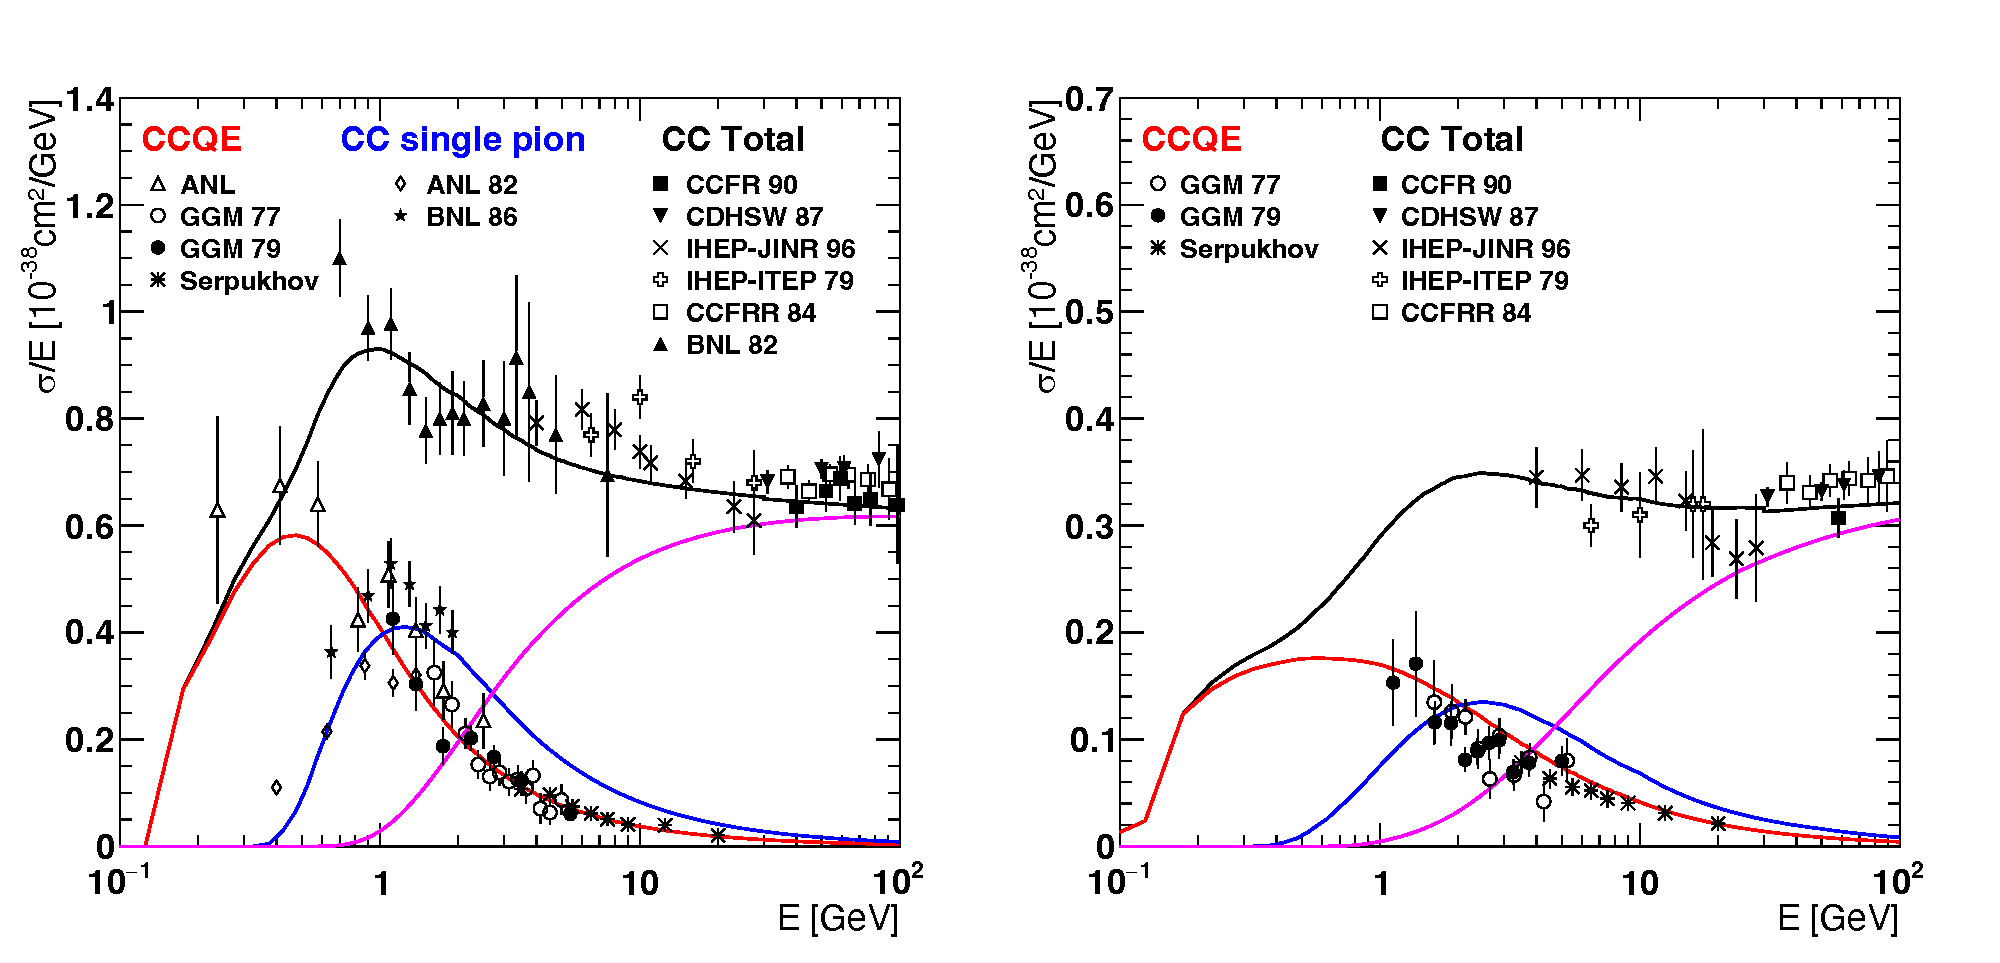
\includegraphics[width=16cm]{Figures/Simulation/CC_XS_numu}
	\caption[Cross sections of charged-current interactions to nucleon for $\nu_{\mu}$ and $\bar{\nu}_{\mu}$ used in NEUT (version 5.4.0.1)]{
	Cross sections of charged-current (CC) interactions to nucleon for $\nu_{\mu}$ (left) and $\bar{\nu}_{\mu}$ (right) used in NEUT (version 5.4.0.1).
	These figures are based on Figure~2 in Ref.~\cite{2020Koshio}.
	Red, blue, and magenta lines show the cross section of CC quasielastic (CCQE) scattering, CC single pion production, and CC deep inelastic scattering, respectively.
	Black line shows the CC total cross section.
	Data plots are taken from the following experiments:
	ANL~\cite{1977Barish}, GGM~77~\cite{1977Bonetti}, GGM~79 (left)~\cite{1979Ciampolillo}, GGM~79 (right)~\cite{1979Armenise}, Serpukhov~\cite{1985Belikov},
	ANL~82~\cite{1982Radecky}, BNL~86~\cite{1986Kitagaki},
	CCFR~90~\cite{1990Auchincloss}, CDHSW~87~\cite{1987Berge}, IHEP-JINR~96~\cite{1996Anikeev}, IHEP-ITEP~79~\cite{1979Mukhin}, CCFRR~84~\cite{1984MacFarlane}, and BNL~82~\cite{1982Baker}.
	}\label{CC_XS_numu}
\end{figure}

\begin{figure}[tbp]
	\centering
	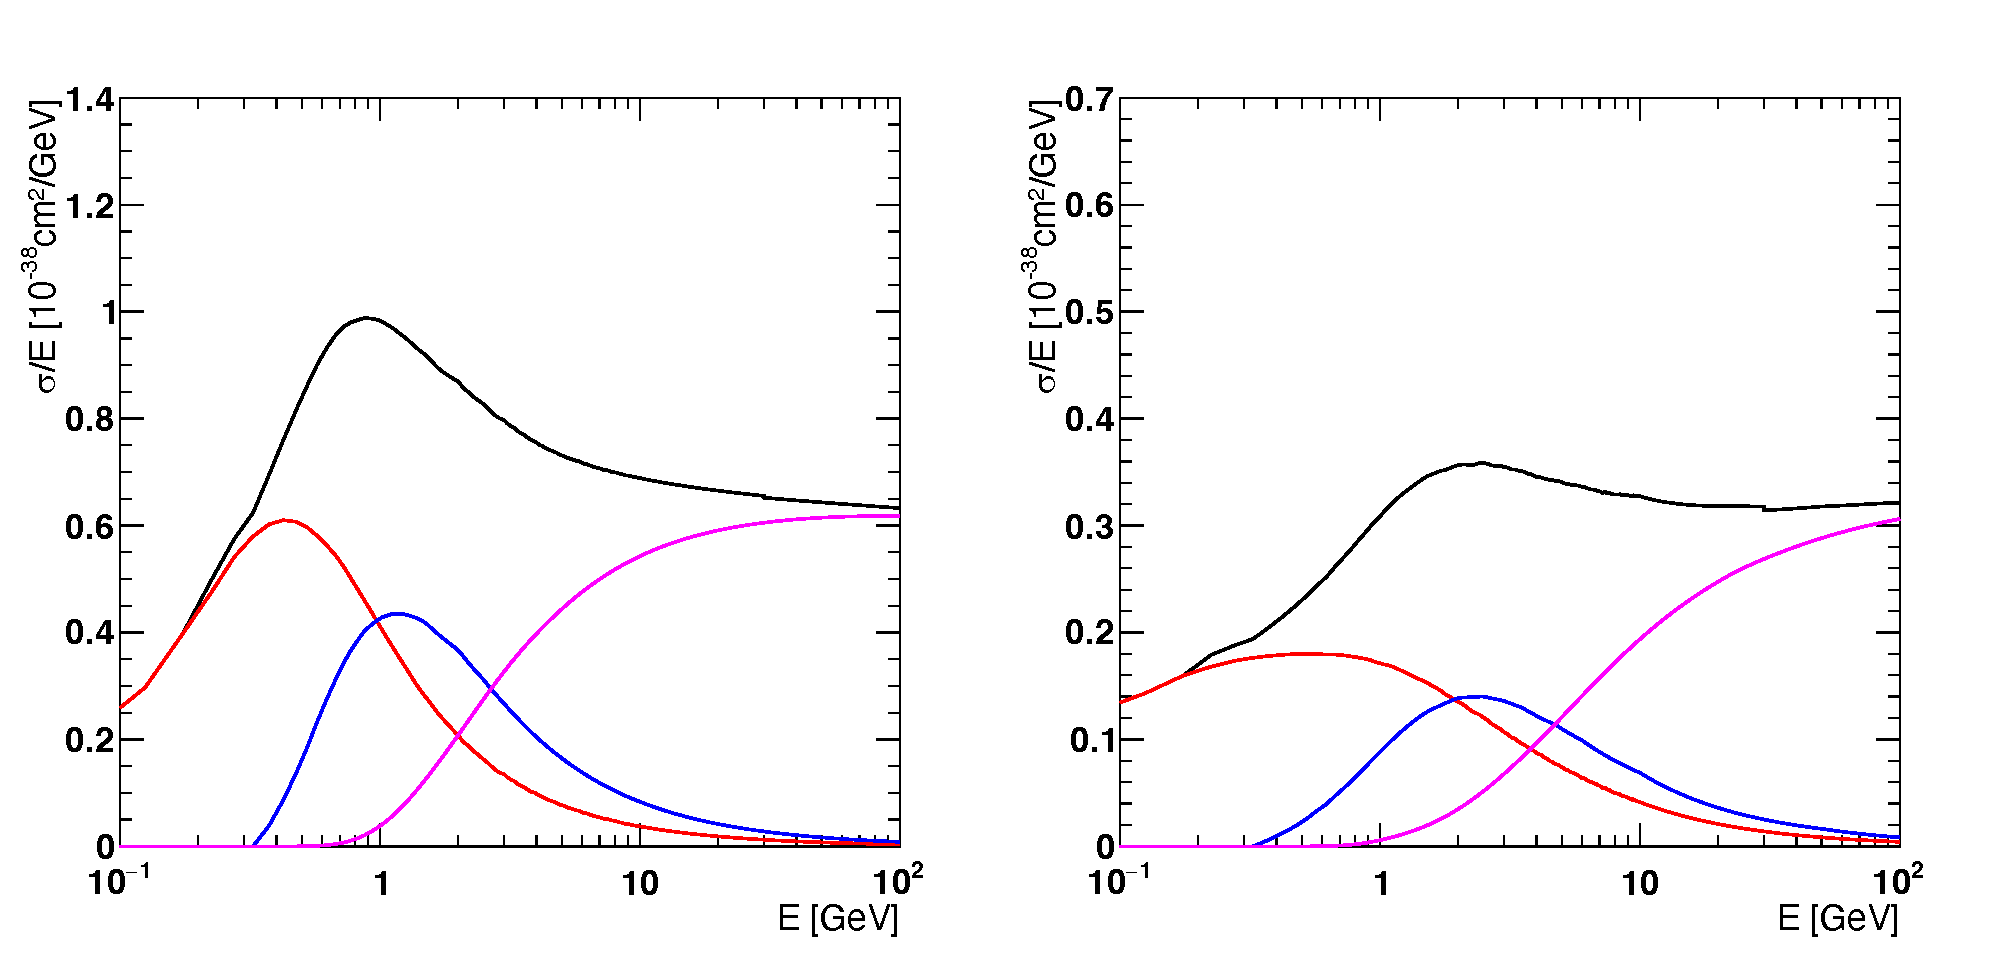
\includegraphics[width=16cm]{Figures/Simulation/CC_XS_nue}
	\caption[Cross sections of charged-current interactions to nucleon for $\nu_{\rm e}$ and $\bar{\nu}_{\rm e}$ used in NEUT (version 5.4.0.1)]{
	Cross sections of charged-current (CC) interactions to nucleon for $\nu_{\rm e}$ (left) and $\bar{\nu}_{\rm e}$ (right) used in NEUT (version 5.4.0.1).
	Red, blue, and magenta lines show the cross section of CC quasielastic (CCQE) scattering, CC single pion production, and CC deep inelastic scattering, respectively.
	Black line shows the CC total cross section.
	}\label{CC_XS_nue}
\end{figure}

\hs
Figure~\ref{NCQE} shows the schematic view of neutrino-oxygen NCQE scattering.
The NCQE cross section on oxygen is based on the model using the oxygen spectral function~\cite{2005Benhar,2012Ankowski} with the BBBA05 vector form factor~\cite{2006Bradford} and the dipole axial form factor~\cite{2006Bradford}.

\begin{figure}[tbp]
	\centering
	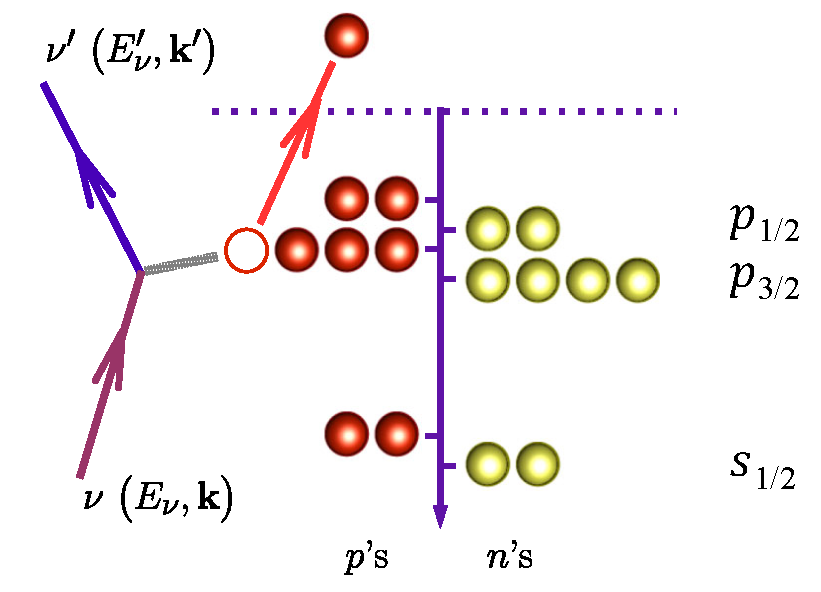
\includegraphics[width=8cm]{Figures/Simulation/NCQE}
	\caption[Schematic view of neutrino-oxygen NCQE scattering]{
	Schematic view of neutrino-oxygen NCQE scattering~\cite{2012Ankowski}.
	Dashed line represents the nucleon emission threshold.
	According to the shell model, protons and neutrons in the $^{16}{\rm O}$ nucleus occupy three states ($p_{1/2}$, $p_{3/2}$, and $s_{1/2}$).
	The removal energy of $p_{1/2}$ state, $p_{3/2}$ state, and $s_{1/2}$ state for protons is 12.1~MeV, 18.4~MeV, and $\sim$42~MeV, respectively.
	The removal energy for neutrons is 3.54~MeV larger than that for protons.
	}\label{NCQE}
\end{figure}

\hs
According to Ref.~\cite{2012Ankowski}, NCQE cross section is defined as
\begin{eqnarray}
	{d^{2}\sigma_{\nu A} \over d\Omega dE^{\prime}_{\nu}}=\sum_{N={\rm p},{\rm n}} \int d^{3}pdEP_{N}(\bm{p}, E){M \over E_{N}}{d^{2}\sigma_{\nu N} \over d\Omega dE^{\prime}_{\nu}},
\end{eqnarray}
where $M$ is the nucleon mass and $E_{N} = \sqrt{M^{2} + \bm{p}^{2}}$.
$P_{N}(\bm{p}, E)$ is the spectral function, that is, the probability of removing a nucleon of momentum $\bm{p}$ from the target leaving the residual nucleus with energy $E+E_{0}-M$, $E_{0}$ being the target ground state energy.
$d^{2}\sigma_{\nu N}/d\Omega dE^{\prime}_{\nu}$ is the neutrino-nucleon cross section.
In the nuclear shell model, the spectral function $P_{N}(\bm{p}, E)$ can be written in the form
\begin{eqnarray}
	P_{N}(\bm{p}, E)=\sum_{\alpha\in\{F\}} n_{\alpha}|\phi_{\alpha}(\bm{p})|^{2}f_{\alpha}(E-E_{\alpha}),
\end{eqnarray}
where $n_{\alpha}$ ($\leq 1$) is the occupation probability of the $\alpha$th state, $\phi_{\alpha}(\bm{p})$ is the momentum-space wave function associated with the $\alpha$th state, $f_{\alpha}(E-E_{\alpha})$ is the (unit-normalized) function describing the energy width of the $\alpha$th state, $-E_{\alpha}$ ($E_{\alpha}>0$) being the binding energy of the $\alpha$th state, and the sum is extended to all occupied states belonging to the Fermi sea $\{F\}$.
The neutrino-nucleon cross section $d^{2}\sigma_{\nu N}/d\Omega dE^{\prime}_{\nu}$ can be written in the form
\begin{eqnarray}
	{d^{2}\sigma_{\nu N} \over d\Omega dE^{\prime}_{\nu}}={G_{F}^{2} \over 8\pi^{2}}{E^{\prime}_{\nu} \over E_{\nu}}{L_{\mu\nu}W^{\mu\nu} \over ME^{\prime}_{N}}\delta(\tilde{\omega}+E_{N}-E^{\prime}_{N}),
\end{eqnarray}
where $G_{F}$ is the Fermi coupling constant and $E^{\prime}_{N} = \sqrt{M^{2} + \bm{p}^{\prime 2}}$.
The leptonic tensor $L_{\mu\nu}$ and the hadronic tensor $W^{\mu\nu}$ are given by
\begin{eqnarray}
	L_{\mu\nu}&=&2(k^{\prime}_{\mu}k_{\nu} + k^{\prime}_{\nu}k_{\mu} - g_{\mu\nu}k \cdot k^{\prime} - i\varepsilon_{\mu\nu\alpha\beta}k^{\alpha}k^{\prime\beta}), \\
	W^{\mu\nu}&=&-g^{\mu\nu}M^{2}W_{1} + \tilde{p}^{\mu}\tilde{p}^{\nu}W_{2} + i\varepsilon^{\mu\nu\alpha\beta}\tilde{p}_{\alpha}\tilde{q}_{\beta}W_{3} + \tilde{q}^{\mu}\tilde{q}^{\nu}W_{4} + (\tilde{p}^{\mu}\tilde{q}^{\nu} + \tilde{p}^{\nu}\tilde{q}^{\mu})W_{5},
\end{eqnarray}
where $\tilde{p}=(E_{N}, \bm{p})$ and $\tilde{q}=(\tilde{\omega}, \bm{k} - \bm{k}^{\prime})$.
The structure functions $W_{i}$ ($i=1,2,3,4,5$) can be written as
\begin{eqnarray}
	W_{1}&=&\tau(\mathcal{F}^{N}_{1} + \mathcal{F}^{N}_{2})^{2} + (1 + \tau)\mathcal{F}^{2}_{A}, \nonumber \\
	W_{2}&=&(\mathcal{F}^{N}_{1})^{2} + \tau(\mathcal{F}^{N}_{2})^{2} + \mathcal{F}^{2}_{A}, \nonumber \\
	W_{3}&=&(\mathcal{F}^{N}_{1} + \mathcal{F}^{N}_{2})\mathcal{F}_{A}, \nonumber \\
	W_{4}&=&{1 \over 4}[(\mathcal{F}^{N}_{1})^{2} + \tau(\mathcal{F}^{N}_{2})^{2} - (\mathcal{F}^{N}_{1} + \mathcal{F}^{N}_{2})^{2} - 4\mathcal{F}_{P}(\mathcal{F}_{A} - \tau\mathcal{F}_{P})], \nonumber \\
	W_{5}&=&{1 \over 2}W_{2},
\end{eqnarray}
where $\tau = -\tilde{q}^{2}/(4M^{2})$.
The nucleon form factors \{$\mathcal{F}^{N}_{i}$ ($i=1,2$), $\mathcal{F}_{A}$, $\mathcal{F}_{P}$\} can be written as
\begin{eqnarray}
	\mathcal{F}^{N}_{1}&=&\pm{1 \over 2}(F^{{\rm p}}_{1} - F^{{\rm n}}_{1}) - 2\sin^{2}\theta_{W}F^{N}_{1}, \nonumber \\
	\mathcal{F}^{N}_{2}&=&\pm{1 \over 2}(F^{{\rm p}}_{2} - F^{{\rm n}}_{2}) - 2\sin^{2}\theta_{W}F^{N}_{2}, \nonumber \\
	\mathcal{F}_{A}    &=&{1 \over 2}{\Delta s \pm g_{A} \over (1 - \tilde{q}^{2}/M_{A}^{2})^{2}}, \nonumber \\
	\mathcal{F}_{P}    &=&{2M^{2}\mathcal{F}_{A} \over m_{\pi}^{2} - \tilde{q}^{2}},
\end{eqnarray}
where the upper (lower) sign corresponds to proton (neutron) form factors, $\theta_{W}$ is the weak mixing angle, $\Delta s$ ($=-0.08$) is the strange quark contribution, $g_{A}=-1.2673$, $M_{A}$ is the axial mass, and $m_{\pi}$ is the pion mass.
The form factors $F^{N}_{1}$ and $F^{N}_{2}$ can be expressed as
\begin{eqnarray}
	F^{N}_{1}&=&{G^{N}_{E} + \tau G^{N}_{M} \over 1 + \tau}, \nonumber \\
	F^{N}_{2}&=&{G^{N}_{M} - G^{N}_{E} \over 1 + \tau},
\end{eqnarray}
where $G^{N}_{E}$ is the electric form factors and $G^{N}_{M}$ is the magnetic form factors.
Figure~\ref{Simula_NCQECroSec} shows the NCQE cross section on nucleon and on oxygen nucleus as a function of neutrino energy.
Figure~\ref{BBBA05} shows the ratio of the BBBA05 vector form factors to $G_{d}$ (the dipole axial form factor).\\
\hs
The state of the residual nucleus after primary interaction (see Figure~\ref{Introd_NCQE_PriSec}) is selected based on the probabilities computed in Ref.~\cite{2012Ankowski}.
There are four states, $(p_{1/2})^{-1}$, $(p_{3/2})^{-1}$, $(s_{1/2})^{-1}$, and \textit{others}, where $($state$)^{-1}$ shows the state of the nucleus after a nucleon initially occupying the state ($p_{1/2}$, $p_{3/2}$, or $s_{1/2}$) is removed.
The production probability of each state is 0.1580, 0.3515, 0.1055, and 0.3850, respectively.
The production probabilities of $(p_{1/2})^{-1}$ state, $(p_{3/2})^{-1}$ state, and $(s_{1/2})^{-1}$ state are obtained by multiplying the spectroscopic strength by the probability that a nucleon in the state is knocked out.
Spectroscopic strengths of the $^{16}{\rm O}$ hole states and probabilities that a nucleon in the state is knocked out are summarized in Table~\ref{Spec}.
The production probability of \textit{others} state is equal to 1~$-$~0.1580~$-$~0.3515~$-$~0.1055.

\begin{figure}[H]
	\centering
	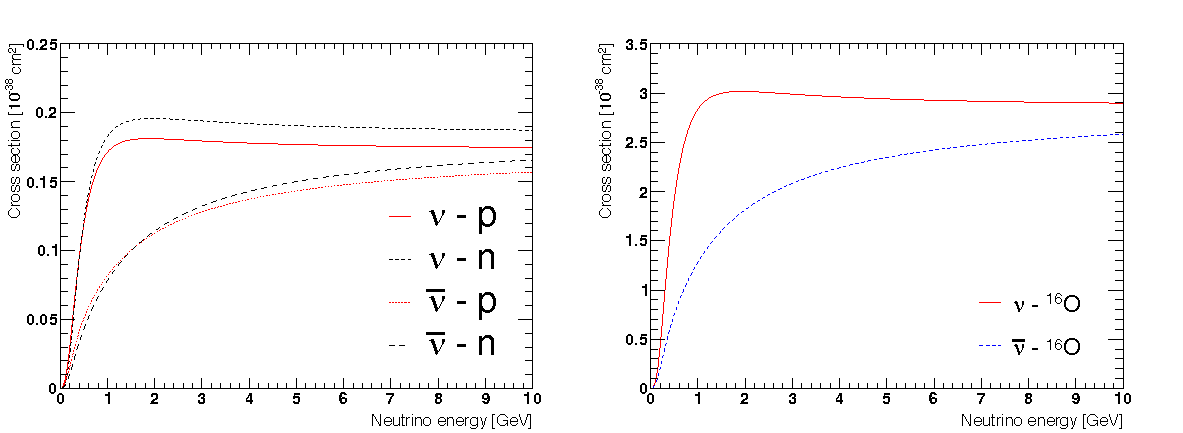
\includegraphics[width=16cm]{Figures/Simulation/NCQECroSec}
	\caption[NCQE cross section on nucleon and on oxygen nucleus as a function of neutrino energy]{
	NCQE cross section on nucleon (left) and on oxygen nucleus (right) as a function of neutrino energy~\cite{2012Ankowski}.
	}\label{Simula_NCQECroSec}
\end{figure}

\begin{figure}[H]
	\centering
	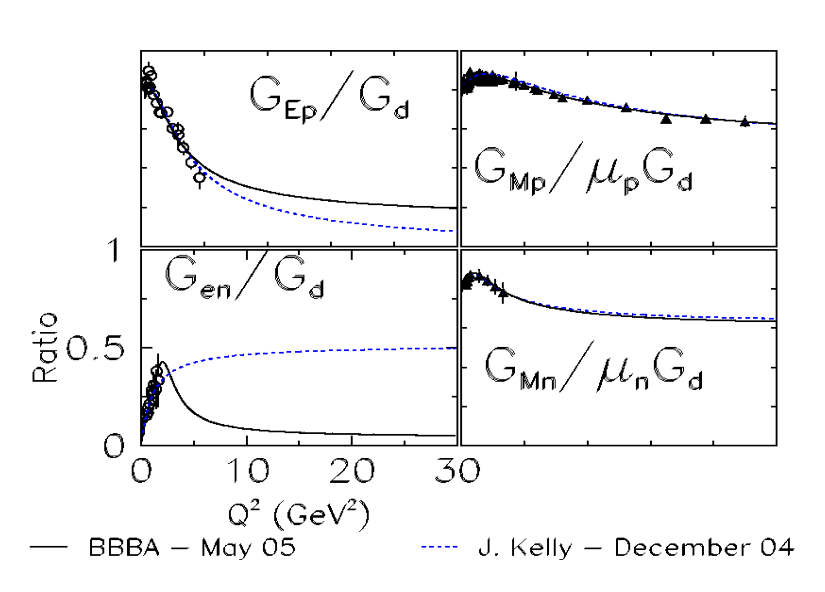
\includegraphics[width=10cm]{Figures/Simulation/BBBA05}
	\caption[The ratio of the BBBA05 vector form factors to $G_{d}$]{
	The ratio of the BBBA05 vector form factors to $G_{d}$ (the dipole axial form factor) (shown in the solid brack line)\cite{2006Bradford}.
	The dashed blue line shows the ratio of the Kelly form factors to $G_{d}$.
	}\label{BBBA05}
\end{figure}

\begin{table}[H]
	\centering
	\caption[Spectroscopic strengths of the $^{16}{\rm O}$ hole states and probabilities that a nucleon in the state is knocked out]{
	Spectroscopic strengths of the $^{16}{\rm O}$ hole states ($S_{\alpha}$) and probabilities that a nucleon in the state is knocked out ($P_{\alpha}$)~\cite{2012Ankowski}.
	}\label{Spec}
	\vs
	\begin{tabular}{lrrr} \hline \hline
		$\alpha$     & $p_{1/2}$ & $p_{3/2}$ & $s_{1/2}$ \\ \hline
		$S_{\alpha}$ & 0.632     & 0.703     & 0.422     \\
		$P_{\alpha}$ & 2$/$8     & 4$/$8     & 2$/$8     \\ \hline \hline
	\end{tabular}
\end{table}

\hs
$(p_{1/2})^{-1}$ state is the ground state of $^{15}{\rm O}$ or $^{15}{\rm N}$, thus no gamma-ray is emitted.
Mainly 6.18~MeV or 6.32~MeV gamma-rays are emitted from $(p_{3/2})^{-1}$ state of $^{15}{\rm O}$ or $^{15}{\rm N}$, respectively~\cite{1994Leuschner,1991Ajzenberg}.
De-excitation modes of $(p_{3/2})^{-1}$ state implemented in NEUT are summarized in Table~\ref{deex_p3_2_O} and Table~\ref{deex_p3_2_N}.
In the case of $(s_{1/2})^{-1}$ state, nucleons and gamma-rays are emitted because the excitation energy is high.
The de-excitation mode is selected based on the $^{16}{\rm O}({\rm p}, 2{\rm p})$ experiment~\cite{2006Kobayashi}.
De-excitation modes of $(s_{1/2})^{-1}$ state implemented in NEUT are summarized in Table~\ref{deex_s1_2_O} and Table~\ref{deex_s1_2_N}.
In the case that the residual nuclei are $^{14}{\rm N}\,+\,{\rm p}$, kinetic energy of generated proton ($E_{{\rm p}}$) is calculated by
\begin{eqnarray}\label{Ep_14Np}
	E_{{\rm p}} = {\rm max}\bigg[0,\,(39.5 \times \eta + 10.65 - E_{l} - E_{^{14}{\rm N}\,+\,{\rm p}}) \times {m_{^{14}{\rm N}} + E_{l} \over m_{{\rm p}} + m_{^{14}{\rm N}} + E_{l}}\bigg],
\end{eqnarray}
where $\eta$ is a random number uniformly distributed in the range from 0 to 1, $E_{l}$ is the energy level, $E_{^{14}{\rm N}\,+\,{\rm p}}$ ($=7.30~{\rm MeV}$) is the energy threshold of two-body decay from $^{15}{\rm O}$ to $^{14}{\rm N}\,+\,{\rm p}$, $m_{^{14}{\rm N}}$ ($=13043.78~{\rm MeV}$) is the mass of $^{14}{\rm N}$ ground state, and $m_{{\rm p}}$ ($=938.27~{\rm MeV}$) is the proton mass.
In the case that the residual nuclei are $^{14}{\rm O}\,+\,{\rm n}$, kinetic energy of generated neutron ($E_{{\rm n}}$) is calculated by
\begin{eqnarray}\label{En_14On}
	E_{{\rm n}} = {\rm max}\bigg[0,\,(39.5 \times \eta + 10.65 - E_{l} - E_{^{14}{\rm O}\,+\,{\rm n}}) \times {m_{^{14}{\rm O}} + E_{l} \over m_{{\rm n}} + m_{^{14}{\rm O}} + E_{l}}\bigg],
\end{eqnarray}
where $E_{^{14}{\rm O}\,+\,{\rm n}}$ ($=13.22~{\rm MeV}$) is the energy threshold of two-body decay from $^{15}{\rm O}$ to $^{14}{\rm O}\,+\,{\rm n}$, $m_{^{14}{\rm O}}$ ($=13048.92~{\rm MeV}$) is the mass of $^{14}{\rm O}$ ground state, and $m_{{\rm n}}$ ($=939.56~{\rm MeV}$) is the neutron mass.
In the case that the residual nuclei are $^{14}{\rm N}\,+\,{\rm n}$, $E_{{\rm n}}$ is calculated by
\begin{eqnarray}\label{En_14Nn}
	E_{{\rm n}} = {\rm max}\bigg[0,\,(39.5 \times \eta + 10.65 - E_{l} - E_{^{14}{\rm N}\,+\,{\rm n}}) \times {m_{^{14}{\rm N}} + E_{l} \over m_{{\rm n}} + m_{^{14}{\rm N}} + E_{l}}\bigg],
\end{eqnarray}
where $E_{^{14}{\rm N}\,+\,{\rm n}}$ ($=10.83~{\rm MeV}$) is the energy threshold of two-body decay from $^{15}{\rm N}$ to $^{14}{\rm N}\,+\,{\rm n}$.
In the case that the residual nuclei are $^{14}{\rm C}\,+\,{\rm p}$, $E_{{\rm p}}$ is calculated by
\begin{eqnarray}\label{Ep_14Cp}
	E_{{\rm p}} = {\rm max}\bigg[0,\,(39.5 \times \eta + 10.65 - E_{l} - E_{^{14}{\rm C}\,+\,{\rm p}}) \times {m_{^{14}{\rm C}} + E_{l} \over m_{{\rm p}} + m_{^{14}{\rm C}} + E_{l}}\bigg],
\end{eqnarray}
where $E_{^{14}{\rm C}\,+\,{\rm p}}$ ($=10.21~{\rm MeV}$) is the energy threshold of two-body decay from $^{15}{\rm N}$ to $^{14}{\rm C}\,+\,{\rm p}$ and $m_{^{14}{\rm C}}$ ($=13043.94~{\rm MeV}$) is the mass of $^{14}{\rm C}$ ground state.
The \textit{others} state includes all other possibilities that are not in $(p_{1/2})^{-1}$, $(p_{3/2})^{-1}$, and $(s_{1/2})^{-1}$ states, and there are no data nor theoretical predictions covered by this state.
In our simulation, the \textit{others} state is set to be integrated into $(s_{1/2})^{-1}$ state by default.\\
\hs
Other distributions related to this section are summarized in Appendix~\ref{App_Simula}.

\begin{table}[H]
	\centering
	\caption[De-excitation modes of $(p_{3/2})^{-1}$ state for $^{15}{\rm O}$ implemented in NEUT]{
	De-excitation modes of $(p_{3/2})^{-1}$ state for $^{15}{\rm O}$ implemented in NEUT.
	$E_{\gamma}$ and $E_{{\rm p}}$ show the (kinetic) energy of generated gamma-ray and generated proton, respectively.
	Probabilities that the mode is selected in NEUT are summarized in the rightmost column.
	Please also check Ref.~\cite{1994Leuschner,1991Ajzenberg}.
	}\label{deex_p3_2_O}
	\vs
	\begin{tabular}{ccccc} \hline \hline
		Residual nuclei            & Energy level  & $E_{\gamma}$  & $E_{{\rm p}}$ & Probability \\
		                           & $({\rm MeV})$ & $({\rm MeV})$ & $({\rm MeV})$ &             \\ \hline
		$^{15}{\rm O}$             & 6.18          & 6.18          & -             & 86.86\%     \\
		$^{14}{\rm N}\,+\,{\rm p}$ & 9.61          & -             & 0.5           & 4.92\%      \\
		$^{14}{\rm N}\,+\,{\rm p}$ & 10.48         & -             & 0.5           & 8.22\%      \\ \hline \hline
	\end{tabular}
\end{table}

\begin{table}[H]
	\centering
	\caption[De-excitation modes of $(p_{3/2})^{-1}$ state for $^{15}{\rm N}$ implemented in NEUT]{
	De-excitation modes of $(p_{3/2})^{-1}$ state for $^{15}{\rm N}$ implemented in NEUT.
	$E_{\gamma}$ and $E_{{\rm p}}$ show the (kinetic) energy of generated gamma-rays and generated proton, respectively.
	Probabilities that the mode is selected in NEUT are summarized in the rightmost column.
	Please also check Ref.~\cite{1994Leuschner,1991Ajzenberg}.
	}\label{deex_p3_2_N}
	\vs
	\begin{tabular}{ccccc} \hline \hline
		Residual nuclei            & Energy level  & $E_{\gamma}$    & $E_{{\rm p}}$ & Probability \\
		                           & $({\rm MeV})$ & $({\rm MeV})$   & $({\rm MeV})$ &             \\ \hline
		$^{15}{\rm N}$             & 6.32          & 6.32            & -             & 86.86\%     \\
		$^{15}{\rm N}$             & 9.93          & 9.93            & -             & 3.82\%      \\
		$^{15}{\rm N}$             & 9.93          & 5.30$\,+\,$4.64 & -             & 0.76\%      \\
		$^{15}{\rm N}$             & 9.93          & 6.32$\,+\,$3.61 & -             & 0.24\%      \\
		$^{15}{\rm N}$             & 9.93          & 7.30$\,+\,$2.63 & -             & 0.10\%      \\
		$^{14}{\rm C}\,+\,{\rm p}$ & 10.70         & -               & 0.5           & 8.22\%      \\ \hline \hline
	\end{tabular}
\end{table}

\begin{table}[h]
	\centering
	\caption[De-excitation modes of $(s_{1/2})^{-1}$ state for $^{15}{\rm O}$ implemented in NEUT]{
	De-excitation modes of $(s_{1/2})^{-1}$ state for $^{15}{\rm O}$ implemented in NEUT.
	$E_{\gamma}$, $E_{{\rm n}}$, and $E_{{\rm p}}$ show the (kinetic) energy of generated gamma-ray, generated neutron, and generated proton, respectively.
	Probabilities that the mode is selected in NEUT are summarized in the rightmost column.
	The last two rows consider the three-body decay of $^{15}{\rm O}$.
	Please also check Ref.~\cite{2006Kobayashi}.
	}\label{deex_s1_2_O}
	\vs
	\begin{tabular}{cccccc} \hline \hline
		Residual nuclei            & Energy level  & $E_{\gamma}$  & $E_{{\rm n}}$            & $E_{{\rm p}}$            & Probability \\
		                           & $({\rm MeV})$ & $({\rm MeV})$ & $({\rm MeV})$            & $({\rm MeV})$            &             \\ \hline
		$^{13}{\rm N}\,+\,{\rm d}$ & 3.09          & 3.09          & -                        & -                        & 3.00\%      \\
		$^{13}{\rm N}\,+\,{\rm d}$ & 3.68          & 3.68          & -                        & -                        & 4.17\%      \\
		$^{13}{\rm N}\,+\,{\rm d}$ & 3.85          & 3.68          & -                        & -                        & 1.67\%      \\
		$^{13}{\rm N}\,+\,{\rm d}$ & 3.85          & 3.85          & -                        & -                        & 2.88\%      \\
		$^{12}{\rm N}\,+\,{\rm t}$ & 4.44          & 4.44          & -                        & -                        & 5.80\%      \\
		$^{14}{\rm N}\,+\,{\rm p}$ & g.s.          & -             & -                        & Equation~(\ref{Ep_14Np}) & 6.74\%      \\
		$^{14}{\rm N}\,+\,{\rm p}$ & 4.92          & 4.92          & -                        & Equation~(\ref{Ep_14Np}) & 5.04\%      \\
		$^{14}{\rm N}\,+\,{\rm p}$ & 5.69          & 3.38          & -                        & Equation~(\ref{Ep_14Np}) & 2.88\%      \\
		$^{14}{\rm N}\,+\,{\rm p}$ & 5.69          & 5.69          & -                        & Equation~(\ref{Ep_14Np}) & 1.62\%      \\
		$^{14}{\rm N}\,+\,{\rm p}$ & 5.83          & 5.11          & -                        & Equation~(\ref{Ep_14Np}) & 0.34\%      \\
		$^{14}{\rm N}\,+\,{\rm p}$ & 5.83          & 5.83          & -                        & Equation~(\ref{Ep_14Np}) & 0.12\%      \\
		$^{14}{\rm N}\,+\,{\rm p}$ & 6.45          & 5.11          & -                        & Equation~(\ref{Ep_14Np}) & 0.23\%      \\
		$^{14}{\rm N}\,+\,{\rm p}$ & 6.45          & 6.44          & -                        & Equation~(\ref{Ep_14Np}) & 1.96\%      \\
		$^{14}{\rm N}\,+\,{\rm p}$ & 7.03          & 7.03          & -                        & Equation~(\ref{Ep_14Np}) & 6.61\%      \\
		$^{14}{\rm O}\,+\,{\rm n}$ & g.s.          & -             & Equation~(\ref{En_14On}) & -                        & 1.15\%      \\
		$^{14}{\rm O}\,+\,{\rm n}$ & 6.73          & 6.73          & Equation~(\ref{En_14On}) & -                        & 0.41\%      \\
		$^{14}{\rm O}\,+\,{\rm n}$ & 7.34          & 6.09          & Equation~(\ref{En_14On}) & -                        & 2.79\%      \\
		$^{14}{\rm O}\,+\,{\rm n}$ & 7.34          & 6.73          & Equation~(\ref{En_14On}) & -                        & 1.96\%      \\
		$^{14}{\rm O}\,+\,{\rm n}$ & 7.34          & 7.34          & Equation~(\ref{En_14On}) & -                        & 0.95\%      \\
		-                          & -             & -             & -                        & 0--5                     & 31.90\%     \\
		-                          & -             & -             & 0--5                     & -                        & 17.78\%     \\ \hline \hline
	\end{tabular}
\end{table}

\begin{table}[h]
	\centering
	\caption[De-excitation modes of $(s_{1/2})^{-1}$ state for $^{15}{\rm N}$ implemented in NEUT]{
	De-excitation modes of $(s_{1/2})^{-1}$ state for $^{15}{\rm N}$ implemented in NEUT.
	$E_{\gamma}$, $E_{{\rm n}}$, and $E_{{\rm p}}$ show the (kinetic) energy of generated gamma-ray, generated neutron, and generated proton, respectively.
	Probabilities that the mode is selected in NEUT are summarized in the rightmost column.
	The last two rows consider the three-body decay of $^{15}{\rm N}$.
	Please also check Ref.~\cite{2006Kobayashi}.
	}\label{deex_s1_2_N}
	\vs
	\begin{tabular}{cccccc} \hline \hline
		Residual nuclei            & Energy level  & $E_{\gamma}$  & $E_{{\rm n}}$            & $E_{{\rm p}}$            & Probability \\
		                           & $({\rm MeV})$ & $({\rm MeV})$ & $({\rm MeV})$            & $({\rm MeV})$            &             \\ \hline
		$^{13}{\rm C}\,+\,{\rm d}$ & 3.09          & 3.09          & -                        & -                        & 3.00\%      \\
		$^{13}{\rm C}\,+\,{\rm d}$ & 3.68          & 3.68          & -                        & -                        & 4.17\%      \\
		$^{13}{\rm C}\,+\,{\rm d}$ & 3.85          & 3.68          & -                        & -                        & 1.67\%      \\
		$^{13}{\rm C}\,+\,{\rm d}$ & 3.85          & 3.85          & -                        & -                        & 2.88\%      \\
		$^{12}{\rm C}\,+\,{\rm t}$ & 4.44          & 4.44          & -                        & -                        & 5.80\%      \\
		$^{14}{\rm N}\,+\,{\rm n}$ & g.s.          & -             & Equation~(\ref{En_14Nn}) & -                        & 6.74\%      \\
		$^{14}{\rm N}\,+\,{\rm n}$ & 4.92          & 4.92          & Equation~(\ref{En_14Nn}) & -                        & 5.04\%      \\
		$^{14}{\rm N}\,+\,{\rm n}$ & 5.69          & 3.38          & Equation~(\ref{En_14Nn}) & -                        & 2.88\%      \\
		$^{14}{\rm N}\,+\,{\rm n}$ & 5.69          & 5.69          & Equation~(\ref{En_14Nn}) & -                        & 1.62\%      \\
		$^{14}{\rm N}\,+\,{\rm n}$ & 5.83          & 5.11          & Equation~(\ref{En_14Nn}) & -                        & 0.34\%      \\
		$^{14}{\rm N}\,+\,{\rm n}$ & 5.83          & 5.83          & Equation~(\ref{En_14Nn}) & -                        & 0.12\%      \\
		$^{14}{\rm N}\,+\,{\rm n}$ & 6.45          & 5.11          & Equation~(\ref{En_14Nn}) & -                        & 0.23\%      \\
		$^{14}{\rm N}\,+\,{\rm n}$ & 6.45          & 6.44          & Equation~(\ref{En_14Nn}) & -                        & 1.96\%      \\
		$^{14}{\rm N}\,+\,{\rm n}$ & 7.03          & 7.03          & Equation~(\ref{En_14Nn}) & -                        & 6.61\%      \\
		$^{14}{\rm C}\,+\,{\rm p}$ & g.s.          & -             & -                        & Equation~(\ref{Ep_14Cp}) & 1.15\%      \\
		$^{14}{\rm C}\,+\,{\rm p}$ & 6.73          & 6.73          & -                        & Equation~(\ref{Ep_14Cp}) & 0.41\%      \\
		$^{14}{\rm C}\,+\,{\rm p}$ & 7.34          & 6.09          & -                        & Equation~(\ref{Ep_14Cp}) & 2.79\%      \\
		$^{14}{\rm C}\,+\,{\rm p}$ & 7.34          & 6.73          & -                        & Equation~(\ref{Ep_14Cp}) & 1.96\%      \\
		$^{14}{\rm C}\,+\,{\rm p}$ & 7.34          & 7.34          & -                        & Equation~(\ref{Ep_14Cp}) & 0.95\%      \\
		-                          & -             & -             & 0--5                     & -                        & 31.90\%     \\
		-                          & -             & -             & -                        & 0--5                     & 17.78\%     \\ \hline \hline
	\end{tabular}
\end{table}





\clearpage
\subsection{Simulation for the IBD-like event}
\vs\hs
Spallation events, reactor neutrino events, and DSNB events are estimated by generating one positron and one neutron isotropically over the entire ID in MC.
Moreover, the positron energy is uniform.
The number of events is later normalized by using neutrino flux or positron (electron) energy spectrum.
Details for the normalization are summarized below.

\subsubsection{Spallation events}\label{Subsubsec_sim_spa}
\vs\hs
Spallation events are decays of radioactive isotopes produced by nuclear spallation of oxygen nuclei induced by energetic cosmic ray muons.
Figure~\ref{Simulation_Spallation_event} shows the schematic view of a spallation event.
Some radioactive isotopes emit one electron and one neutron, mimicing the IBD events.
Most of them can be ignored due to a short lifetime and a low yield, however, $^{9}{\rm Li}$ cannot be ignored because of a relatively long lifetime ($\sim$0.26~s) and a large yield ($1.9 \times 50.8\% \times 10^{-7} \mu^{-1}g^{-1}{\rm cm}^{2}$)~\cite{2007Battistoni}.
Therefore, the number of events is normalized by using the energy spectrum of electrons from $^{9}{\rm Li}$ decays and the measured $^{9}{\rm Li}$ rate at SK ($0.86\,\pm\,0.12 ({\rm stat.})\,\pm\,0.15 ({\rm syst.})\,{\rm kton}^{-1}{\rm day}^{-1}$)~\cite{2015Zhang}.
Figure~\ref{9Li_ene} shows the energy spectrum of electrons from $^{9}{\rm Li}$ decays modeled by the BESTIOLE code~\cite{2010ThomasPhD}.

\begin{figure}[H]
	\centering
	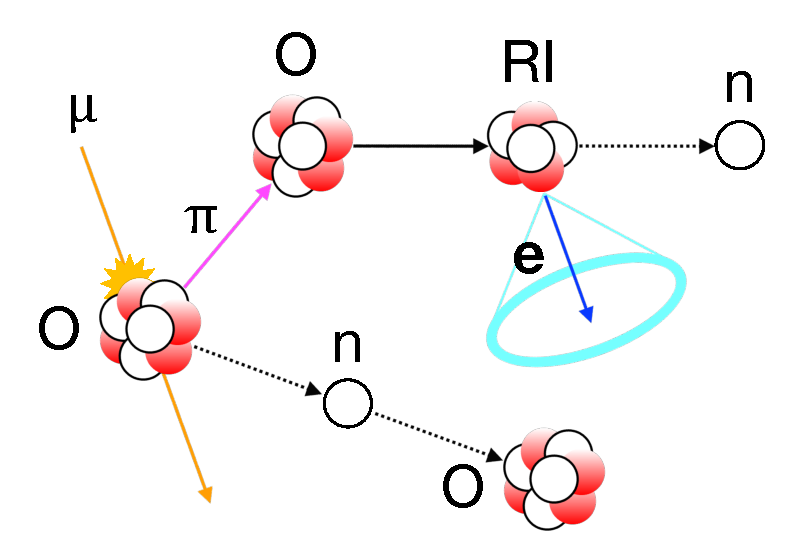
\includegraphics[width=6cm]{Figures/Simulation/Spallation_event}
	\caption[Schematic view of a spallation event]{
	Schematic view of a spallation event.
	RI stands for radioactive isotope.
	}\label{Simulation_Spallation_event}
\end{figure}

\begin{figure}[H]
	\centering
	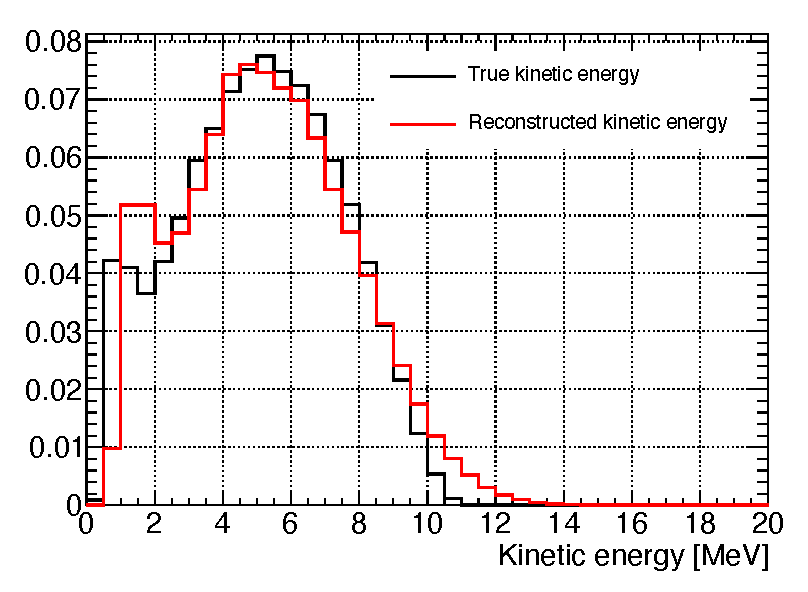
\includegraphics[width=8cm]{Figures/Simulation/9Li_ene}
	\caption[Energy spectrum of electrons from $^{9}{\rm Li}$ decays modeled by the BESTIOLE code]{
	Energy spectrum of electrons from $^{9}{\rm Li}$ decays modeled by the BESTIOLE code~\cite{2010ThomasPhD,2023HaradaPhD}.
	Red line shows the reconstructed energy spectrum.
	}\label{9Li_ene}
\end{figure}

\subsubsection{Reactor neutrino events}\label{Subsubsec_sim_reactor}
\vs\hs
While reactors are operating, many electron antineutrinos are generated via beta decays.
Reactor neutrino events are also the IBD events by electron antineutrinos from reactors.
The reactor neutrino flux is calculated using SKReact\footnote{If you would like to know how to use SKReact, please check the url (\url{https://github.com/Goldie643/SKReact}).}, which is a tool for calculating the electron antineutrino flux from reactors, considering the activity of each reactor near the SK.
Figure~\ref{Reactor_act} shows the activities of Japanese reactors from April 2018.
The number of events is normalized by using the reactor neutrino flux (shown in Figure~\ref{Reactor_flux}) and the IBD cross section of Strumia-Vissani model~\cite{2003Strumia} (shown in Figure~\ref{IBD_XS}).

\begin{figure}[H]
	\centering
	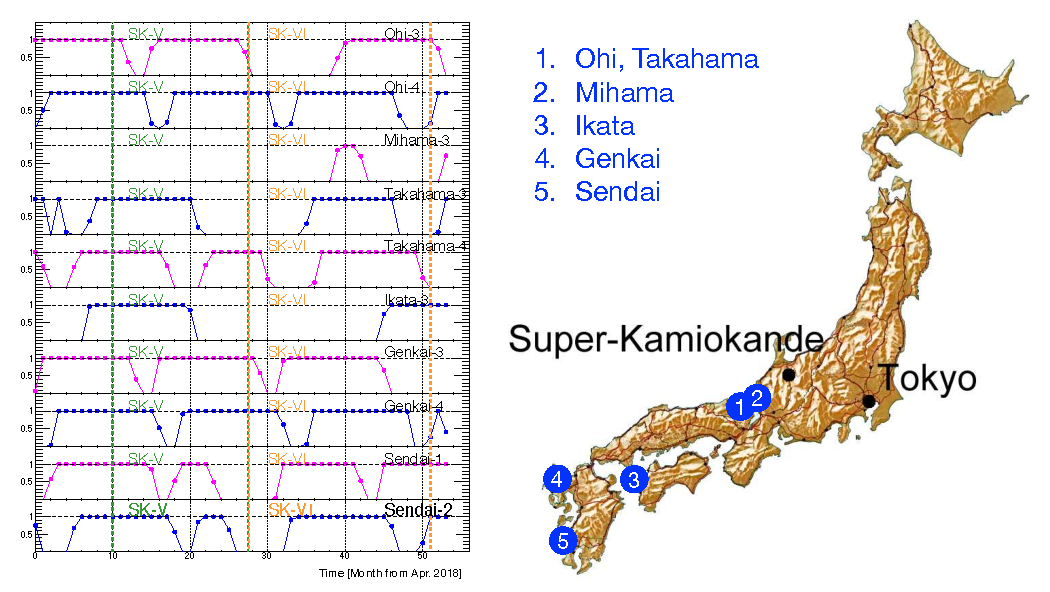
\includegraphics[width=12cm]{Figures/Simulation/Reactor_act}
	\caption[Activities of Japanese reactors from April 2018]{
	Activities of Japanese reactors from April 2018~\cite{2003Fukuda,2023HaradaPhD}.
	Dashed line shows the 100\% operation.
	Locations of nuclear power plants, Tokyo, and the SK are also shown in right side.
	}\label{Reactor_act}
\end{figure}

\begin{figure}[H]
	\centering
	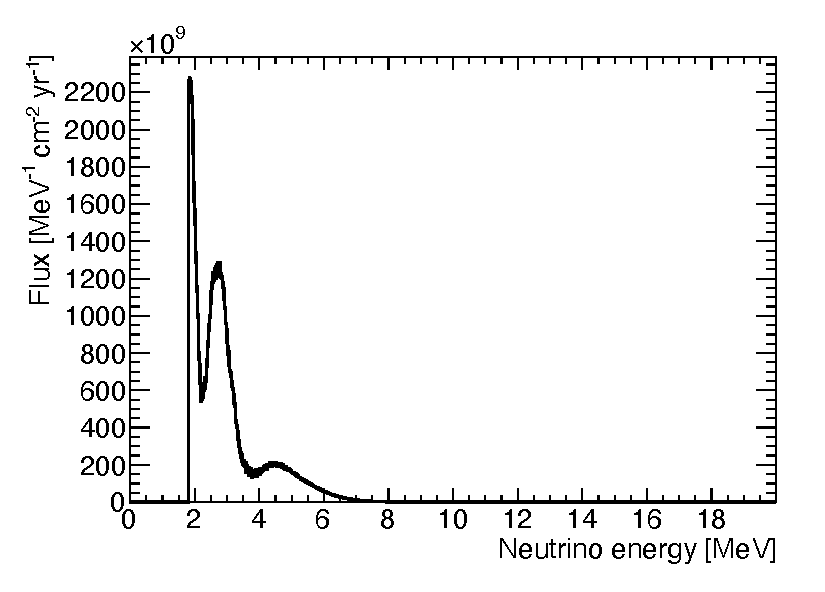
\includegraphics[width=8cm]{Figures/Simulation/Reactor_flux}
	\caption[Expected reactor neutrino flux at the SK]{
	Expected reactor neutrino flux at the SK~\cite{2023HaradaPhD}.
	In this flux, neutrino oscillation effect is considered.
	}\label{Reactor_flux}
\end{figure}

\begin{figure}[H]
	\centering
	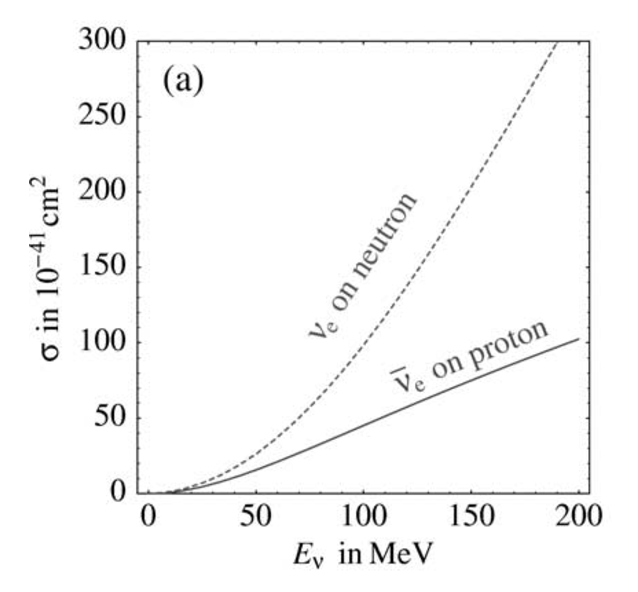
\includegraphics[width=6cm]{Figures/Simulation/IBD_XS}
	\caption[IBD cross section of Strumia-Vissani model]{
	IBD cross section of Strumia-Vissani model~\cite{2003Strumia}.
	}\label{IBD_XS}
\end{figure}

\subsubsection{DSNB events}
\vs\hs
As described in Section~\ref{Subsec_DSNBsearch}, DSNB events are the IBD events by electron antineutrinos.
The number of events is normalized by using the DSNB electron antineutrino flux (shown in Figure~\ref{Introd_DSNBpred}) and the IBD cross section of Strumia-Vissani model~\cite{2003Strumia} (shown in Figure~\ref{IBD_XS}).





\subsection{Detector simulation}
\vs\hs
In the past, a GEANT3-based~\cite{1994Brun} SK detector simulation (SKDETSIM, SK Detector Simulation) where only the Bertini Cascade Model (BERT) was implemented for neutron tracking in water was used.
However, a Geant4-based~\cite{2016Allison} (version 10.05.p01) SK detector simulation (SKG4, Super-Kamiokande Geant4 based Simulation) has been newly developed for the SK-Gd experiment.
In this simulation, BERT ({\tt \verb|FTFP_BERT_HP|} physics list), the Binary Cascade Model (BIC) ({\tt \verb|QGSP_BIC_HP|} physics list), and the Li$\grave{\text{e}}$ge Intranuclear Cascade model (INCL++) ({\tt \verb|QGSP_INCLXX_HP|} physics list) can be used as the secondary interaction model.
Here, BERT is a traditional cascade model used in GEANT.
BIC uses a large set of hadron data to choose interaction processes to improve the accuracy.
INCL++ is an advanced binary cascade model including phase space and quantum mechanical processes.
The features of each secondary interaction model are described in Section~\ref{Subsec_Features}.
In this NCQE cross section measurement, BERT is used as the baseline model.\\
\hs
Figure~\ref{model_ninel}, Figure~\ref{model_pinel}, and Figure~\ref{model_piinel} show the final state models of inelastic scattering for neutron, proton, and charged pion, respectively.
As described in Section~\ref{Subsec_NCQEbackground}, knocked-out neutrons of NCQE events may have hundreds of MeV, and neutrons with hundreds of MeV follow BERT, BIC, or INCL++ model as shown in Figure~\ref{model_ninel}.
Therefore, it is important to understand the difference among these models and select an appropriate model.\\
\hs
As shown in Figure~\ref{model_piinel}, when the kinetic energy (momentum) of incoming charged pion is below 379.544~(500)~MeV, NEUT model is used.
At the energy range, cross sections of charged pion inelastic scattering are also replaced to those of NEUT.
Figure~\ref{XS_piinel} shows the cross sections of charged pion inelastic scattering.\\
\hs
Gamma-rays emitted from thermal neutron capture on Gd are based on ANNRI-Gd model~\cite{2020Tanaka}.
Here, ANNRI stands for the Accurate Neutron-Nucleus Reaction Measurement Instrument.
Figure~\ref{Simula_RatioGdGam} shows the ratio of data from the ANNRI experiment to MC with the ANNRI-Gd model for the single gamma-ray events~\cite{2020Tanaka}.
As shown in this figure, the ANNRI-Gd model shows good agreement with the data.

\begin{figure}[H]
	\centering
	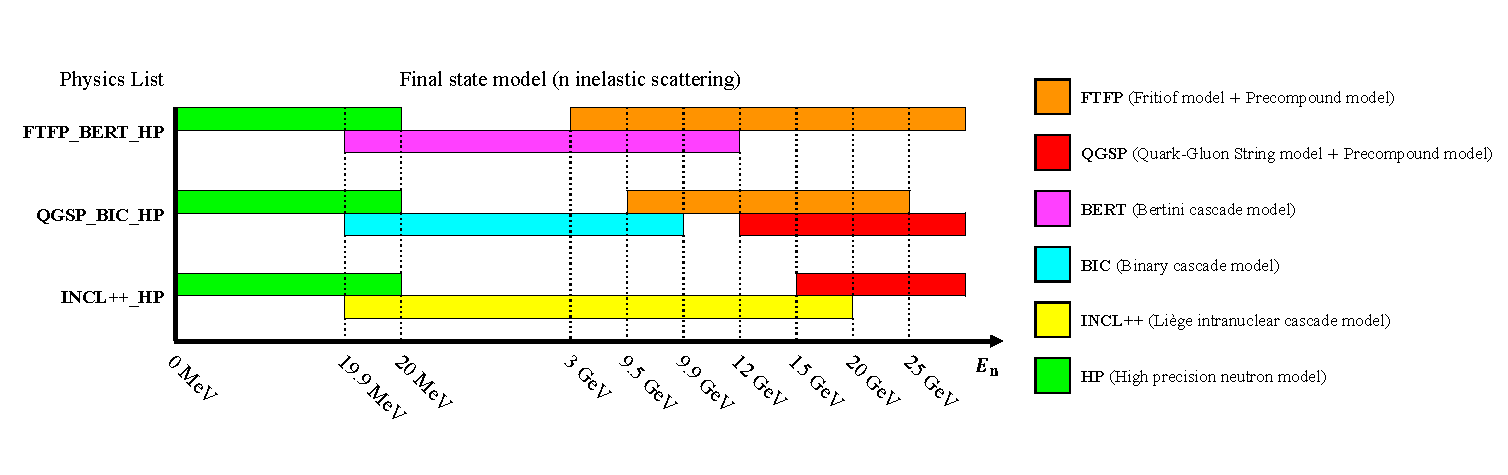
\includegraphics[width=16cm]{Figures/Simulation/model_ninel}
	\caption[Final state models of neutron inelastic scattering]{
	Final state models of neutron inelastic scattering.
	Horisontal axis represents the kinetic energy of incoming neutron.
	}\label{model_ninel}
\end{figure}

\begin{figure}[H]
	\centering
	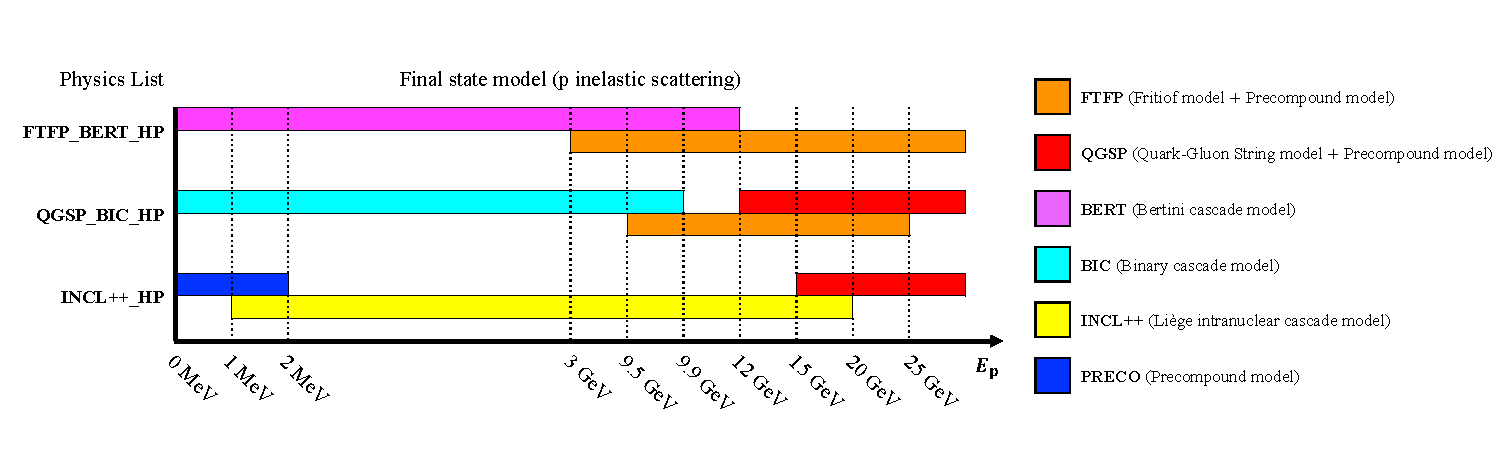
\includegraphics[width=16cm]{Figures/Simulation/model_pinel}
	\caption[Final state models of proton inelastic scattering]{
	Final state models of proton inelastic scattering.
	Horisontal axis represents the kinetic energy of incoming proton.
	}\label{model_pinel}
\end{figure}

\begin{figure}[H]
	\centering
	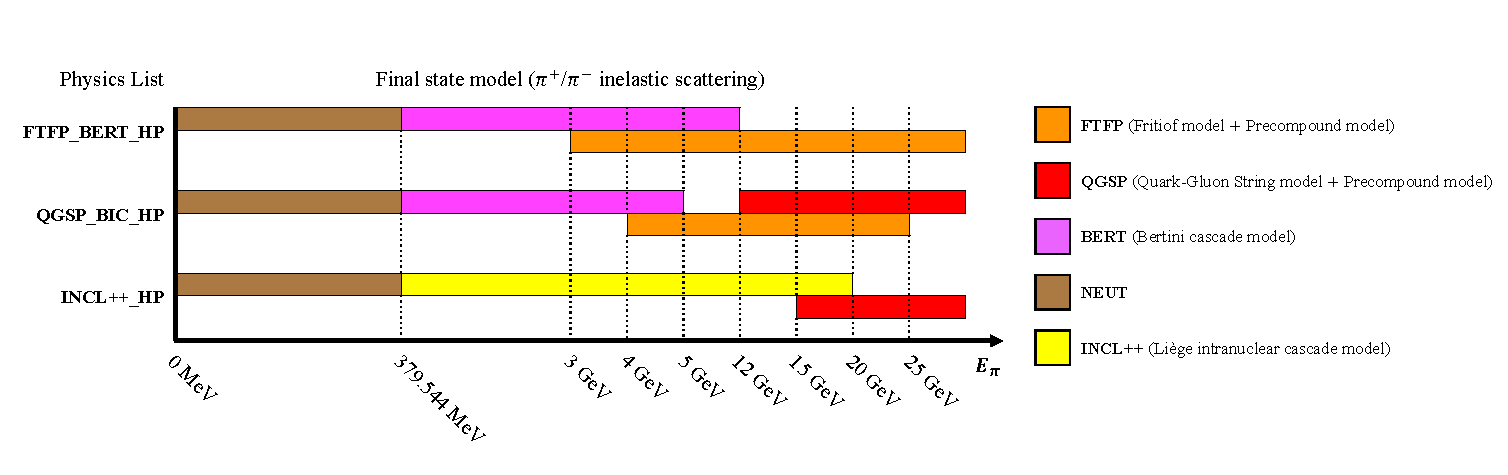
\includegraphics[width=16cm]{Figures/Simulation/model_piinel}
	\caption[Final state models of charged pion inelastic scattering]{
	Final state models of charged pion inelastic scattering.
	Horisontal axis represents the kinetic energy of incoming charged pion.
	}\label{model_piinel}
\end{figure}

\begin{figure}[tbp]
	\centering
	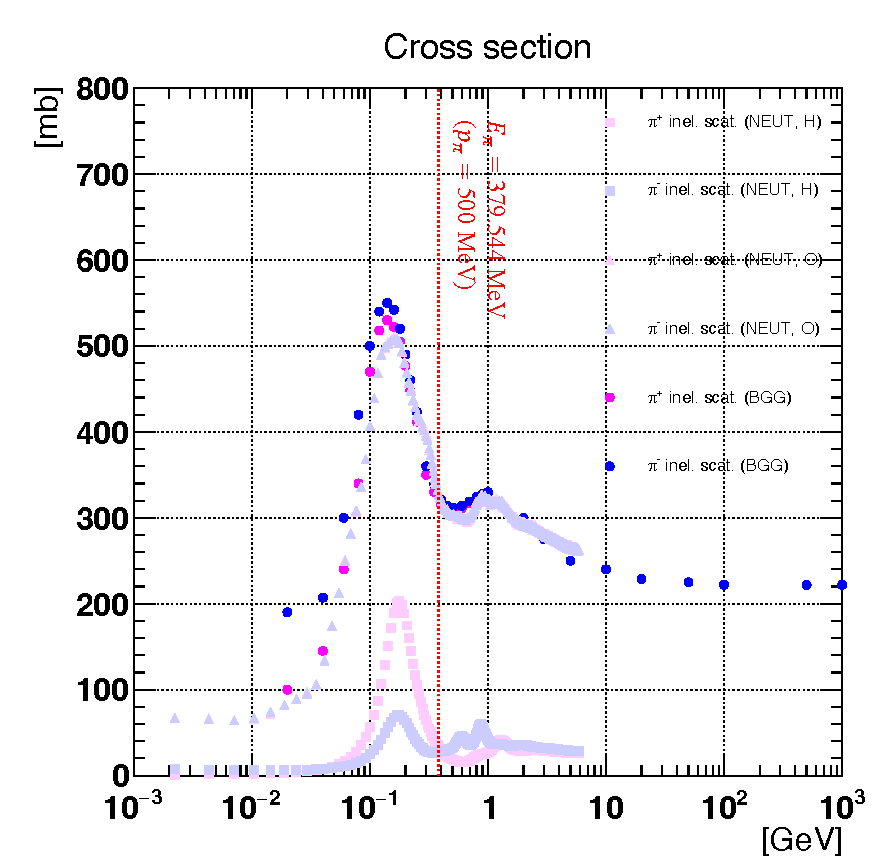
\includegraphics[width=10cm]{Figures/Simulation/XS_piinel}
	\caption[Cross sections of charged pion inelastic scattering]{
	Cross sections of charged pion inelastic scattering.
	Horisontal axis shows the kinetic energy of incoming charged pion.
	BGG stands for Barashenkov-Glauber-Gribov.
	}\label{XS_piinel}
\end{figure}

\begin{figure}[tbp]
	\centering
	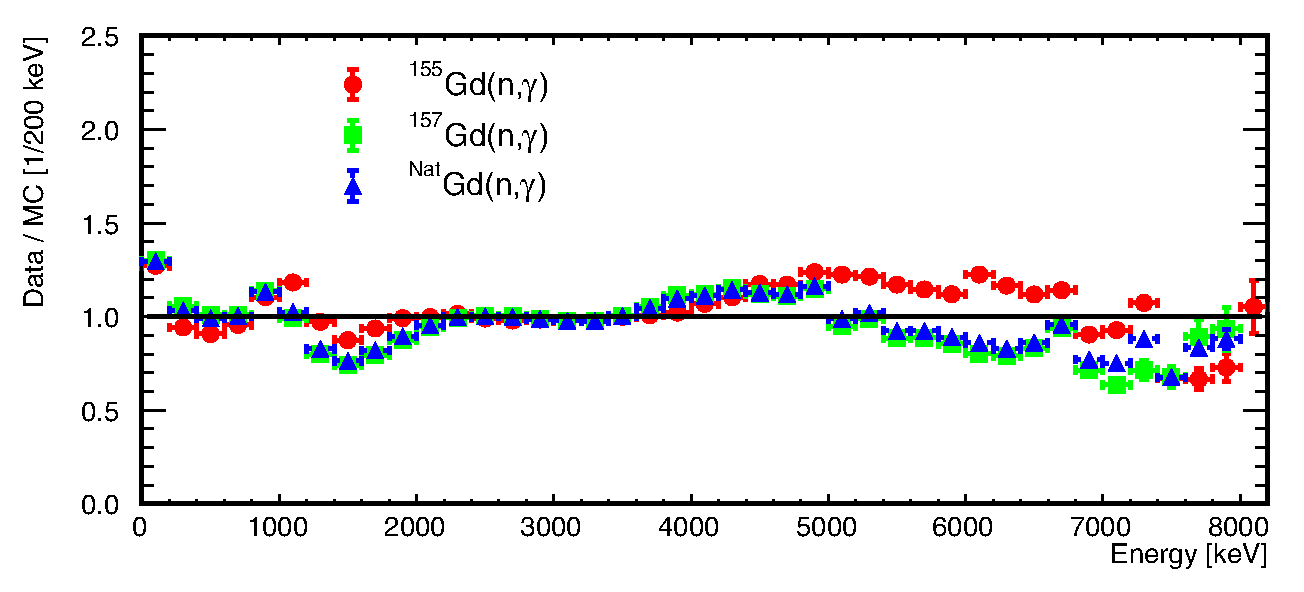
\includegraphics[width=10cm]{Figures/Simulation/RatioGdGam}
	\caption[Ratio of data from the ANNRI experiment by MC with the ANNRI-Gd model for the single gamma-ray events]{
	Ratio of data from the ANNRI experiment to MC with the ANNRI-Gd model for the single gamma-ray events~\cite{2020Tanaka}.
	}\label{Simula_RatioGdGam}
\end{figure}





\newpage

